\documentclass[..thesis.tex]{subfiles}


\tikzstyle{component} = [rectangle, rounded corners = 5pt, inner sep  = 5pt, draw=black, text width=2.5cm, text centered]

\tikzstyle{arrow} = [thick,->,>=stealth]

\lstdefinestyle{caml}{
	showstringspaces=false,
        language=Caml,
        literate=
               {->}{$\rightarrow$}{1},
        morekeywords ={module, sig, val, include},
        emph = [1]{int, bool, unit, list, option}, emphstyle=[1]{\textit},
        emph = [2]{varinfo, exp, lval, fundec}, emphstyle=[2]{\underline} 
}





\begin{document}

\toguide{What is the point here?}

In this section, we give an overview  of \textit{Goblint}, a static analyzer for race detection in C programs with focus on Linux device drivers that has been developed for over 10 years in University of Tartu and in the Technical University of Munich.

\toadd{Cite the arctile written, doctorial thesis of Kalmer and Vesal, github repo}

\toask{Should cite something else?}

\toguide{Why are we intrested in Goblint?}

The original work presented in this thesis builds on top done on Goblint. The background information given in this section will hopefully enable one to put that into context.

\tosup{So keep in mind that this is the main objective! I will give some comments, but you should also go through each paragraph of this section and ask if it helps provide context to the next section or is just distracting details.}
\toguide{Okay, got it. So, what is Goblint?}

Goblint is a constraint system based analysis tool, that performs abstract interpretation, building on top of the ideas described in previous section. Goblint is written in OCaml and is publicly available on Github.

\toadd{check that it is previous section.}

as an input, Goblint takes a $c$ program and uses the CIL framework to process it into intermediate form that can then be converted into control flow graph (\textit{cfg}). 

\toadd{cite CIL}

as a next step, the enabled \textit{analyses specifications} are combined and a constraint system that corresponds to the combined analyses and \textit{cfg} of the program is produced.

the generated constraint system in then solved with a generic constraint system solver. 

finally, the output is mapped to the original $c$ program and displayed to user in a suitable format.

\begin{figure}[H]
  \centering
  \begin{tikzpicture}[node distance = 2.5cm and 1.5cm]
    \node (cil) [component] {CIL preprocessor};
    \node (cfg) [component, below of=cil] {control flow graph constructor};
    \node (conssyst) [component, below of = cfg] {constraint system constructor} ;
    \node (analyses) [component, right  =of conssyst] {analyses combiner};
    \node (analysesb) [component, right  =of analyses] {analyses b};
    \node (analysesa) [component, above of = analysesb] {analyses a};
    \node (analysesrest) [component, below of = analysesb] {$\ldots$};
    \node (analyzer) [component, below of = conssyst] {analyzer};
    \node (generic) [component, right  =of analyzer] {generic constraint system solver};
    \node (output) [component, below of = analyzer] {output formatter};

    \draw [arrow] (cil) -- (cfg);
    \draw [arrow] (cfg) -- (conssyst);
    \draw [arrow] (conssyst) -- (analyzer);
    \draw [arrow] (analyzer) -- (output);
    
    \draw [arrow] (analyses) -- (conssyst);
    
    \draw [arrow] (analysesa) -- (analyses);
    \draw [arrow] (analysesb) -- (analyses);
    \draw [arrow] (analysesrest) -- (analyses);

    \draw [arrow] (generic) -- (analyzer);

  \end{tikzpicture}
  \caption{The structure of Goblint}
\end{figure}


\toguide{Okay, do we need to understand all of it?}

The most interesting components of Goblint are the provided solvers for the constraint systems and the wide array of analyses provided. We will be focusing on the structure of an analyses using as an example the mutex analyses that makes use of the previously discussed ideas of lockset analyses -- this will hopefully both introduce one of the key analyses for Goblint and give an high level idea of how an implementation of an analyses looks like. In addition, we will briefly touch the region analyses that we will use as a building block later on. 

\toadd{Thesis of Kalmer and Vesal, something else?}
The solvers implemented in Goblint do not fall into scope of this thesis. An thorough overview can be found from ...

\toguide{So, how does an analyses look like?}

As previously described, for each analyses, we need an abstract domain to perform the abstract interpretation on. In Goblint, all the domains implement interface Lattice. The functions \textit{join} and \textit{meet} correspond to binary least upper bound and greatest lower bound operations.  


\begin{lstlisting}[language=Caml,style=caml]
module type Lattice =
sig
  include Printable
  val leq: t -> t -> bool
  val join: t -> t -> t
  val meet: t -> t -> t
  val bot: unit -> t
  val is_bot: t -> bool
  val top: unit -> t
  val is_top: t -> bool
  ...
end
\end{lstlisting}

The Lattice type includes module type Printable, that defines, in addition to the shown functions, a set of functions that enable conversion of type t to strings with different format. The type t in Ocaml module type leaves the type abstract. The types written in italic are built-in types in OCaml. 

\tosup{I would not talk about Printable, so I suggest just inlining the type t into the Lattice. Maybe also remove is\_top \& is\_bot. Say somewhere on top that these are simplified/partial signatures.}


\begin{lstlisting}[language=Caml,style=caml]
module type Printable =
sig
  type t
  val equal: t -> t -> bool
  val hash: t -> int
  val compare: t -> t -> int
  ...
end
\end{lstlisting}

In case of the lockset analyses, the domain is reversed set domain of all the possible locks. That is, the elements in the domain are sets of locks in the program under analyses and join operation is defined as the intersection of two sets and meet as union of two sets. The reasoning behind the set domain being reversed is that we are interested in the set off all the locks that must be held at a specific statement. In a situation where we have to take an upper bound of two locksets (say, after two branches of an if-else statement merge), we hence want it to only consist of locks that were in both of the locksets.

Analyses in Goblint must implement the module type Spec. Following is the simplified version of the

\toask{Did I not cover something important? Or something left is maybe not important in context of thesis? Left out: sync, intrpt, }
\toans{No, and I think you can remove more, such as exitstate \& otherstate, but this signature seems okay to me.}

\begin{lstlisting}[language=Caml,style=caml]
module type Spec =
sig
  module D : Lattice
  module G : Lattice

  val name : string

  val startstate : varinfo -> D.t
  val exitstate  : varinfo -> D.t
  val otherstate : varinfo -> D.t

  val part_access: (D.t, G.t) ctx -> exp -> varinfo option -> bool -> (Access.LSSSet.t * Access.LSSet.t)

  val query : (D.t, G.t) ctx -> Queries.t -> Queries.Result.t

  val assign: (D.t, G.t) ctx -> lval -> exp -> D.t
  val branch: (D.t, G.t) ctx -> exp -> bool -> D.t
  val body  : (D.t, G.t) ctx -> fundec -> D.t
  val return: (D.t, G.t) ctx -> exp option  -> fundec -> D.t

  val special : (D.t, G.t) ctx -> lval option -> varinfo -> exp list -> D.t

  val enter   : (D.t, G.t) ctx -> lval option -> varinfo -> exp list -> (D.t * D.t) list
  val combine : (D.t, G.t) ctx -> lval option -> exp -> varinfo -> exp list -> D.t -> D.t

  ...

end
\end{lstlisting}

Here the underscored types are the ones defined in the CIL library.

Each analyses includes two lattices, lattice $D$ will contain the abstract states and lattice $G$ will contain abstract values for global variables.

The type \textit{ctx} with type parameters $\lp D.t, G.t \rp$ encapsulates the both the local and global state, offering access to helper functions on them. 

The functions \textit{startstate},\textit{exitstate} and \textit{otherstate} provide an initial abstract state for a thread depending on whether the thread starts an
initialization function (in context of device drivers, the function that registers the driver and exposes the callback functions),
a cleanup function (where deregistration happens in device drivers) or it is any other function that can be used to spawn a new thread (all the file operations).

The functions take as argument information about the function declaration, enabling Goblint to differentiate between different file operations.
In case of mutex analyses, all the functions always return empty locksets.

The \textit{part\_access} function enables one partition accesses into disjoint groups -- if two accesses to variable $x$ are in different partition then they cannot race.
In addition, it also associates a set of locks held with the partition. This function return empty sets in case of mutex analyses as it does not make use of partitioning,
unlike, for example, the region analyses.
\tosup{This function is important and maybe deserves more explanations, or you should at least highlight (forward-ref perhaps) that this function is what you had to interface with and plays an important role for this thesis.}

The \textit{query} function enables communication between different analyses that have have been combined into one and are being performed at the same time -- 
the analyses must be able to answer the query based on the current context. This allows analyses to avoid duplication and allows one to design more modular analyses consisting of sub-analyses. More regarding the query system of Goblint can be found here \toadd{Cite Kalmer}.

The functions \textit{assign}, \textit{branch}, \textit{body} and \textit{return} are functions from abstract state to abstract state, for assignment statements,
branching statments and for entering and exiting from function calls. They corresponding to the $\lllb s \rrrb^{*}$ family of functions introduced in previous section.

\toadd{Confirm previous.} 

In the implementation for mutex analyses, those transfer functions do not actually change the abstract state as none of the statements do influence the set of locks held.
However, they do register accesses to variables, for example, an access in registered for both the left and right hand side of an assignment with further distinction
that the access to the left hand side is a write access.

The \textit{special} function handles functions for what the source code is not available for Goblint to analyze. In mutex analyses,
 this function modifies the abstract state -- functions calls to functions such as \textit{\_\_raw\_lock\_unlock} and \textit{\_lock\_kernel} 
remove and add mutexes to the set of held locks.

\toadd{Enter and combine, makes sense if I had this to theoretical part as well}

\toguide{Okay, pretty dense stuff. You mentioned region analyses?}
\tosup{This is a pretty big shift in tone from internals to a conceptual description of the analysis. I think both are needed, but it's pretty bad structurally. I might even suggest merging region analysis with your conceptual description of your own contribution and put all implementation details after that chapter where you describe goblint as is and show what changes you made.}

Lastly, another analyses that the author would like to briefly introduce is the region analyses.

\toguide{Okay, what is the point of it?}

Consider a hash table using chaining to handle hash collisions that has a lock for each of the buckets.

\toask{Just one figure with the hash keys shown in good enough?}

\begin{figure}[H]
  \centering
  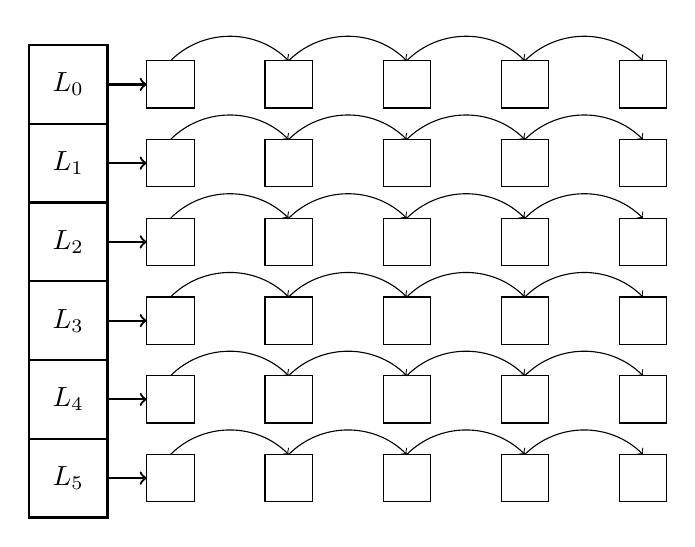
\begin{tikzpicture}
    \foreach \y in {0,...,5}
      {
        \draw[thick]  (0,5 - \y) rectangle  ++(1,1) node[midway] {$L_{\y}$};
        \draw[->, thick] (1,5 - \y + 0.5) -- ++(0.5,0);
        \foreach \x in {1,...,5}
        {
          \draw (1.5*\x, 5 -\y+0.2) rectangle ++(0.6,0.6);

        }
        \foreach \x in {1,...,4}
        {
          \draw[->] (1.5*\x + 0.3, 5 - \y + 0.8) to [bend left=45] ++(1.5,0);
        }
      }
  \end{tikzpicture}
  \caption{Separate chaining hash table} 
\end{figure}
An usual way to synchronize such an hash table is to protect each bucket with its own lock -- if the hashes of the keys $k_1$ and $k_2$ are different then accessing them in the hash table cannot cause a data race. On the other hand, if $k_1$ and $k_3$ produce the same hash then there is a real risk for data race.


\begin{figure}[H]
  \centering
  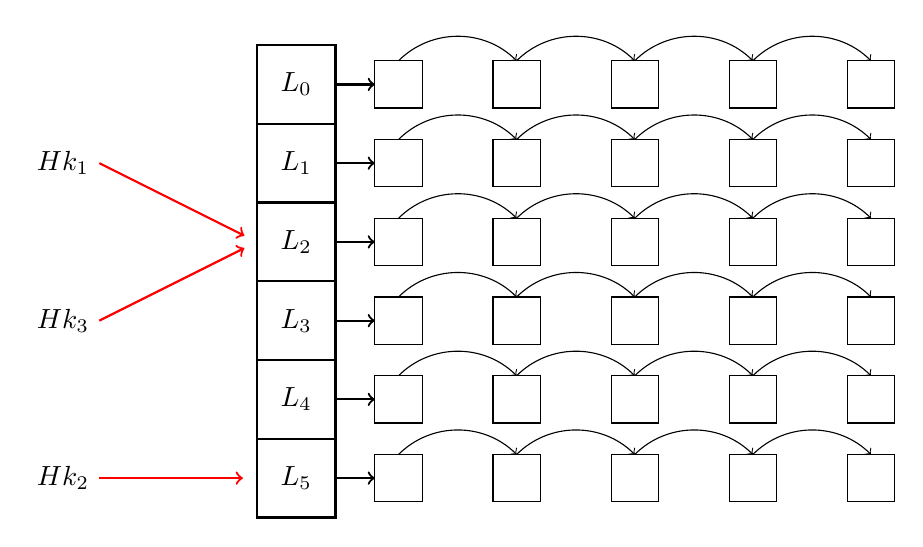
\begin{tikzpicture}
    \foreach \y in {0,...,5}
      {
        \draw[thick]  (0,5 - \y) rectangle  ++(1,1) node[midway] {$L_{\y}$};
        \draw[->, thick] (1,5 - \y + 0.5) -- ++(0.5,0);
        \foreach \x in {1,...,5}
        {
          \draw (1.5*\x, 5 -\y+0.2) rectangle ++(0.6,0.6);

        }
        \foreach \x in {1,...,4}
        {
          \draw[->] (1.5*\x + 0.3, 5 - \y + 0.8) to [bend left=45] ++(1.5,0);
        }
      }
    \draw[red, ->, shorten >= 5pt, thick] (-2,2.5) node [black, anchor =  east] {$H\lp k_3 \rp$} -- (0,3.5);
    \draw[red, ->, shorten >= 5pt, thick] (-2,0.5) node [black, anchor =  east] {$H\lp k_2 \rp$} -- (0,0.5); 
    \draw[red, ->, shorten >= 5pt, thick] (-2,4.5) node [black, anchor =  east] {$H\lp k_1 \rp$} -- (0,3.5);
      
  \end{tikzpicture}
  \caption{Separate chaining hash table} 
\end{figure}


The way region analyses is able to detect that cannot be a data race between additions of an element to hash table with for key $k_1$ and $k_3$ we need to be able to divide the memory that the program uses into disjoint \textit{regions} such that we can guarantee that memory accesses in different regions cannot race.

In case of the hash table, the most obvious partition for the regions would be to separate the buckets of the hash table.


\begin{figure}[H]
  \centering
    \begin{tikzpicture}

      
      \tikzset{xzp/.style={canvas is xz plane at y=#1}}

      \pgfmathsetmacro{\cubex}{10}
      \pgfmathsetmacro{\cubey}{5}
      \pgfmathsetmacro{\cubez}{5}


      \foreach \x in {1,...,5} 
      {
        \draw[thick,dashed] (\x*\cubex*0.2,0,0) -- ++(0,0,\cubez);
      }

      \fill[opacity=0.8,red!30,draw=black,xzp=0] (0,0) rectangle (0.2*\cubex,\cubez);
      \fill[opacity=0.8,blue!40,draw=black,xzp=0] (0.2*\cubex,0) rectangle (0.4*\cubex,\cubez);
      \fill[opacity=0.8,green!40,draw=black,xzp=0] (0.4*\cubex,0) rectangle (0.6*\cubex,\cubez);
      \fill[opacity=0.8,yellow!50!red,draw=black,xzp=0] (0.6*\cubex,0) rectangle (0.8*\cubex,\cubez);
      \fill[opacity=0.8,cyan!40,draw=black,xzp=0] (0.8*\cubex,0) rectangle (\cubex,\cubez);

      \node at (0.275*\cubex,0,0.4*\cubez) (p) {$H \lp k_1 \rp$};
      \node at (0.3*\cubex,0,0.75*\cubez) (q) {$H \lp k_3 \rp$};

      \node at (0.9*\cubex,0,0.35*\cubez) (q) {$H \lp k_2 \rp$};


      \draw[thick,-] (0,0,0)  -- ++(0,0,\cubez) --  node [anchor = north] {$R_1$} ++(0.2*\cubex,0,0) -- node [anchor = north] {$R_2$} ++(0.2*\cubex,0,0) -- node [anchor = north] {$R_3$} ++(0.2*\cubex,0,0) -- node [anchor = north] {$R_4$} ++(0.2*\cubex,0,0) -- node [anchor = north] {$R_5$} ++(0.2*\cubex,0,0)  --  ++(0,0,-\cubez) -- ++(-\cubex,0,0);
    \end{tikzpicture}
    \caption{Memory partition of the hash table}
\end{figure}

The partitioning of memory in a such way is done in Goblint by the region analyses. More information regarding the ideas used can be found ... \toadd{Cite Vesal}

With that we have given a quick overview of Goblint and how an analyses is implemented in it. In addition, a quick overview of a region analyses was given, that we use as bases in the next section.

\end{document}
